\thispagestyle{empty}
\pagecolor{bg}
\text{}
\vfill
\noindent
\begin{minipage}[t]{0.35\textwidth}
	\begin{flushright}
		\textcolor{goban}{\large
			\\
			井蛙不可以語於海者，\\
			拘於虛也；\\[0.5em]
			夏蟲不可以語於冰者，\\
			篤於時也；\\[0.5em]
			曲士不可以語於道者，\\
			束於教也。
		}
	\end{flushright}
\end{minipage}%
\hfill
{\color{goban}\vrule}
\hfill
\begin{minipage}[t]{0.48\textwidth}
	\vspace{1pt}
	\raggedright
	\emph{
		$\!\!$\textcolor{goban}{A frog in a well cannot be spoken to about the ocean\\
			because it is confined by its own space.\\[0.5em]
			A summer insect cannot be spoken to about ice \\
			because it is bound by its own season.\\[0.5em]
			A narrow-minded person cannot be spoken to about the Way \\
			because they are bound by their own teachings.}
	}
\end{minipage}

\vspace{1em}
\hfill {\textcolor{goban}{秋水 — \textsc{Zhuāngzǐ, Chapter 17}}}
\vfill
\begin{center}
	\begin{tikzpicture}[scale=3]
		\definecolor{bpbg}{HTML}{0B2450}
		\definecolor{textcolor}{HTML}{efce8f}
		\definecolor{sealred}{HTML}{9E2A2B}
		\definecolor{goban}{HTML}{efce8f}
		\begin{axis}[
			hide axis,
			view={4}{45},
			axis equal image,
			samples=20,
			domain=0:360,
			y domain=0:360,
			z buffer=sort,
			]
		
			% toro
			\addplot3[
			surf,
			shader=flat,
			fill=bpbg,  
			draw=textcolor,   
			line width=0.4pt,
			opacity=1
			]
			(
			{(2 + cos(y)) * cos(x)},
			{(2 + cos(y)) * sin(x)},
			{sin(y)}
			);
			
			
			%%%%%%%%%%%%%%%%%%%%  hoshi
			\addplot3[
			only marks,
			xslant=-0.15,
			yslant=-0.5,
			mark options={shading=ball, ball color=white},
			opacity=1,
			mark size=0.4pt,
			shading=ball,
			color=goban
			] coordinates {(1.190, 3.94, 0)};
			
			\addplot3[
			only marks,
			mark options={shading=ball, ball color=white},
			opacity=1,
			mark size=0.65pt,
			shading=ball,
			color=goban
			] coordinates {(-1.96, 0.675, 0)};
			
			\addplot3[ %centro
			only marks,
			mark options={shading=ball, ball color=white},
			opacity=1,
			mark size=0.65pt,
			shading=ball,
			color=goban
			] coordinates {(0.975, -0.61, 0)};
			
			\addplot3[ %arriba derecha
			only marks,
			yslant=0.25,
			mark options={shading=ball, ball color=white},
			opacity=1,
			mark size=0.65pt,
			shading=ball,
			color=goban
			] coordinates {(1.09, 1, 0)};
			
			\addplot3[ %abajo derecha
			only marks,
			yslant=0.5,
			opacity=1,
			mark options={shading=ball, ball color=black},
			mark size=0.65pt,
			shading=ball,
			color=goban
			] coordinates {(1.870,-6.179, 0)};
			% 3. Sello 
			\node[
			fill=sealred,
			scale=0.5,
			draw=textcolor,
			line width=0.4pt,
			inner sep=3pt,
			rounded corners=1pt,
			font=\fontsize{12}{12}\selectfont,
			text=textcolor,
			text opacity=1
			] at (axis cs: 0, 0, 0) {復};
		\end{axis}
	\end{tikzpicture}
\end{center}
\vfill
\newpage
\pagecolor{white}

{\centering\chapter{Abstraction}\label{parte3}}
\thispagestyle{empty}
\section{Comparing Adjacencies}\label{chap:6}

Observing the two-dimensional board in Figure~\ref{fig: tableronm}, we can note that it will have \(xy\) intersections; however, the following question arises: how many adjacencies do all these intersections possess?
\begin{figure}[H]
	\centering   
	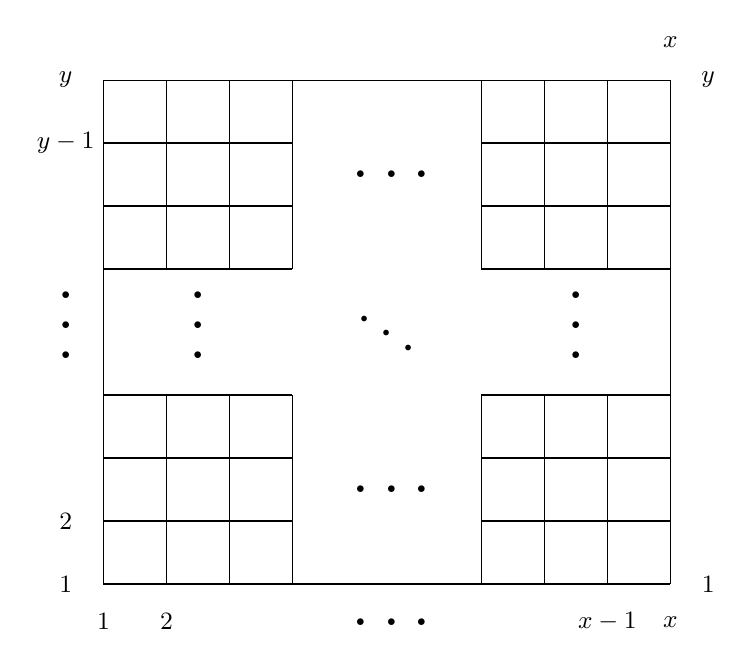
\begin{tikzpicture}[scale=0.8]
		%Cuadrado grande
		\draw (0,0) -- (0,-8);
		\draw (0,0) -- (9,0);
		\draw (9,0) -- (9,-8);
		\draw (0,-8) -- (9,-8);
		%Cuadrado grande
		%Texto horizontal%
		\node(draw)at (0,-8.6) {$1$};
		\node(draw)at (1,-8.6) {$2$};
		\node(draw)at (8,-8.6) {$x-1$};
		\node(draw)at (9,0.6) {$x$};
		\node(draw)at (9.6,0) {$y$};
		
		%Texto vertical%
		\node(draw)at (-0.6,0) {$y$};
		\node(draw)at (-0.6,-1){$y-1$};
		
		\node(draw)at (-0.6,-3.895){\rotatebox{90}{\Huge$\dots$}};
		
		\node(draw)at (-0.6,-7){$2$};
		\node(draw)at (-0.6,-8){$1$};
		%\rotate
		%Lineas para centrar bien
		%\draw (0,-4) -- (9,-4);
		%\draw (4.5,0) -- (4.5,-8);
		%Texto diagonal
		\node(draw)at (9,-8.6) {$x$};
		\node(draw)at (9.6,-8) {$1$};
		\draw[step=1cm] (0,0) grid (3,-3);
		\node(draw)at (1.5,-3.895){\rotatebox{90}{\Huge$\dots$}};
		\node(draw)at (4.526,-3.895) {\rotatebox{-15}
			{\Huge$\ddots$}};
		\node(draw)at (4.573,-8.6) {\Huge$\dots$};
		\node(draw)at (7.5,-3.895) {\rotatebox{90}{\Huge$\dots$}};
		\draw[step=1cm] (0,-5) grid (3,-8);
		\node(draw)at (4.573,-1.5) {\Huge$\dots$};
		\node(draw)at (4.573,-6.5) {\Huge$\dots$};
		\draw[step=1cm] (6,0) grid (9,-3);
		\draw[step=1cm] (6,-5) grid (9,-8);
		
	\end{tikzpicture}
	\caption{Go board of size $x\times y$.}
	\label{fig: tableronm}
\end{figure}
By Lemma~\ref{lem:2n}, for $x, y \ge 2$, these nodes have $2$, $3$, or $4$ adjacencies. The $4$ vertices possess $2$ adjacencies. There are four edges—two of length \((x-2)\) and two of length \((y-2)\)—whose nodes have $3$ adjacencies. Furthermore, there is an internal region of \((x-2)(y-2)\) nodes, each with $4$ adjacencies. This allows us to compute the sum of vertex degrees (total directed adjacencies) on a \(\mathrm{Go}^{2}\) board.

Let \(A(x,y) = \sum_{t \in G} |K(t)|\) be the total number of directed adjacencies on a board of dimensions \(x\times y\) ($x, y \ge 2$).
\begin{align*}
	A(x,y)&= 2\cdot4 + 3(2(x-2))+3(2(y-2))+4(x-2)(y-2)\\
	A(x,y)&= 8 + 6x-12+6y-12+4xy-8x-8y+16\\
	A(x,y)&= 4xy-2x-2y.
\end{align*}
Let us also define the average number of adjacencies (average degree) on a board, which follows immediately from the definition of total adjacencies; it suffices to divide by the total number of nodes.

Let \(\tilde{A}(x,y)\) be the average number of liberties of a single stone on a two-dimensional board, then:
\begin{align*}
	\tilde{A}(x,y)= \frac{4xy-2x-2y}{xy}.
\end{align*}
\subsection{Go in Three Dimensions}

Let us consider the case for \(\mathrm{Go}^3\), consisting of \(xyz\) nodes ($x, y, z \ge 2$). To this end, we rely on the following diagram, Figure~\ref{fig:3dim_esquema} (left):
\begin{figure}[H]
	\centering
	\begin{tikzpicture}[scale=1]
		\pgfmathsetmacro{\x}{-5}
		\pgfmathsetmacro{\y}{6}
		\pgfmathsetmacro{\z}{1.5}
		\path (0,0,\y) coordinate (A) (\x,0,\y) coordinate (B) (\x,0,0) coordinate (C) (0,0,0)
		coordinate (D) (0,\z,\y) coordinate (E) (\x,\z,\y) coordinate (F) (\x,\z,0) coordinate (G)
		(0,\z,0) coordinate (H);
		\draw (A)-- (B)-- (C)--(G)--(F)-- (B) (A)--(E)--(F)--(G)--(H)--(E);
		\draw [dashed,black] (A)--node[below,sloped]{y} (D)-- node[above,sloped]{x}(C) (D)--node[right]{z} (H);
		
		%nodo y sus aristas
		\draw[YellowOrange, ultra thick] (-5,1.5) -- (-5.3,1.2);%adentro
		\draw[YellowOrange, ultra thick]  (-5,1.5) -- (-4.6,1.5);%derecha
		\draw[YellowOrange, ultra thick] (-5,1.5) -- (-5,1.1); %abajo
		
		\fill[color=black] (-5,1.5) circle (0.07);
		\begin{scope}[xshift=7cm]
			\pgfmathsetmacro{\x}{-5}
			\pgfmathsetmacro{\y}{6}
			\pgfmathsetmacro{\z}{1.5}
			\path (0,0,\y) coordinate (A) (\x,0,\y) coordinate (B) (\x,0,0) coordinate (C) (0,0,0)
			coordinate (D) (0,\z,\y) coordinate (E) (\x,\z,\y) coordinate (F) (\x,\z,0) coordinate (G)
			(0,\z,0) coordinate (H);
			\draw (A)-- (B)-- (C)--(G)--(F)--(B) (A)--(E)--(F)--(G)--(H)--(E);
			\draw [black] (A)--(D)--(C) (D)--(H);
			\draw [sealred, ultra thick, |-|](-4.85,0) -- node[above] {$x-2$}(-0.15,0);
			\draw [bg, ultra thick, |-|](-0.15,-0.15) -- node[below,sloped] {$y-2$}(-2.2,-2.2);
			\draw [Moss, ultra thick, |-|](0,1.35) -- node[right] {$z-2$}(0,0.15);
			
			%nodo y sus aristas
			\draw[YellowOrange, ultra thick] (-2,1.5) -- (-2.35,1.15); %adentro
			\draw[YellowOrange, ultra thick]  (-2,1.5) -- (-1.6,1.5); %derecha
			\draw[YellowOrange, ultra thick]  (-2,1.5) -- (-2.4,1.5); %izquierda
			\draw[YellowOrange, ultra thick]  (-2,1.5) -- (-2,1.1);   %abajo
			\fill[color=black] (-2,1.5) circle (0.07);
		\end{scope}
	\end{tikzpicture}
	\caption{Exterior of the three-dimensional board. A vertex with $3$ adjacencies, edges, and a node with $4$ adjacencies.}
	\label{fig:3dim_esquema}
\end{figure}

Proceeding as before, we observe that it possesses $8$ vertices, each with $3$ adjacencies. We identify $4$ edges of \((x-2)\) nodes, $4$ of \((y-2)\), and $4$ of \((z-2)\), each with nodes possessing $4$ adjacencies, see Figure~\ref{fig:3dim_esquema} (right).

Next, we have the faces. These are divided into three pairs: $2$ faces of \((x-2)(y-2)\), $2$ of \((x-2)(z-2)\), and $2$ of \((y-2)(z-2)\), with nodes possessing $5$ adjacencies each, Figure~\ref{fig:3gocaras}.

\begin{figure}[H]
	\centering
	\begin{tikzpicture}[scale=1.1]
		\pgfmathsetmacro{\x}{-5}
		\pgfmathsetmacro{\y}{6}
		\pgfmathsetmacro{\z}{1.5}
		
		%Cara xy
		\filldraw[fill=bg!50!sealred, draw=black,opacity=0.5] (-0.2,-0.1,0) -- (-5,-0.1,0) -- (-4.9,0,5.8) -- (-0.1,0,5.8) -- cycle;
		
		%Cara yz
		\filldraw[fill=Moss!50!bg, draw=black,opacity=0.5](-5.3,-0.2,5) -- (-5.05,0.1,0.1) -- (-5.05,1.35,0.1) -- (-5.3,1.1,5) -- cycle;
		
		%Cara xz
		\filldraw[fill=sealred!50!Moss, draw=black,opacity=0.5] (-0.1,0.1,0) -- (-0.1,1.4,0) -- (-4.9,1.4,0) -- (-4.9,0.1,0) -- cycle;
		
		\draw [black, thin, |-|](-4.9,1.5) -- node[above,sloped] {$(x-2)(z-2)$}(-0.1,1.5);
		\draw [black, thin, |-|](-0.15,-0.15) -- node[below,sloped] {$(x-2)(y-2)$}(-2.29,-2.29);
		\draw [black, thin, |-|](-5.125,1.375) -- node[above,sloped] {$(y-2)(z-2)$}(-7.275,-0.775);
		
		\path (0,0,\y) coordinate (A) (\x,0,\y) coordinate (B) (\x,0,0) coordinate (C) (0,0,0)
		coordinate (D) (0,\z,\y) coordinate (E) (\x,\z,\y) coordinate (F) (\x,\z,0) coordinate (G)
		(0,\z,0) coordinate (H);
		\draw (A)-- (B)--  (C)--(G)--(F)--(B) (A)-- (E)--(F)--(G)--(H)--(E);
		\draw [dashed,black] (A)--(D)--(C) (D)--(H);
		
		
		%nodo y sus aristas
		\draw[YellowOrange, ultra thick] (-2,0.8) -- (-2.4,0.8); %izquierda
		\draw[YellowOrange, ultra thick] (-2,0.8) -- (-1.6,0.8); %derecha
		\draw[YellowOrange, ultra thick]  (-2,0.8) -- (-2,1.2); %arriba
		\draw[YellowOrange, ultra thick] (-2,0.8) -- (-2,0.4); %abajo
		\fill[color=black] (-2,0.8) circle (0.07);
		\draw[YellowOrange, ultra thick]  (-2,0.8) -- (-2.35,0.45); %adentro
		
	\end{tikzpicture}
	\caption{Faces of the three-dimensional board with a node of $5$ adjacencies.}
	\label{fig:3gocaras}
\end{figure}

Remaining is the internal volume, which consists of \((x-2)(y-2)(z-2)\) nodes, each with $6$ adjacencies. We are thus in a position to define the total number of directed adjacencies on a three-dimensional board. 

Let \(A(x,y,z)\) be the number of directed adjacencies of a three-dimensional board, then, we can calculate the adjacencies of any three-dimensional board as follows:
$$
A(x,y,z)=6 x y z - 2 x y - 2 x z - 2 y z.
$$   
And its average,
$$
\tilde{A}(x,y,z)=\frac{6 x y z - 2 x y - 2 x z - 2 y z}{xyz}.
$$
In turn, for $x, y, z \ge 3$, we can define the \textit{exterior} of the three-dimensional board; let \(A(x,y,z)_{\partial}\) be the number of adjacencies of a board of dimensions \(x, y, z\) that only takes the exterior into account. As seen previously, it suffices to sum the vertices, the edges, and, in the case of the faces, we no longer count the adjacency pointing toward the interior, since it ceases to exist as there are no interior nodes, such that our faces have $4$ adjacencies, hence:
$$
A(x,y,z)_{\partial}=8 (x y + x z - 2 x + y z - 2 y - 2 z + 3).
$$
We define the average by subtracting the nodes we are not considering; let \(\tilde{A}(x,y,z)_{\partial}\) be the average number of liberties on the exterior of a board of dimensions \(x, y, z\):
$$
\tilde{A}(x,y,z)_{\partial}=\frac{8 (x y + x z - 2 x + y z - 2 y - 2 z + 3)}{(xyz)-(x-2)(y-2)(z-2)}.
$$
\subsection{Comparing Average Adjacencies}\label{key:libprom}

Prior to the development of this work, as a Go player, I wondered whether a three-dimensional version of the game existed. Upon finding only conceptual images on the Internet, I asked myself: why not develop it? Thus, \href{https://github.com/10500x/3dGo}{3dGo} was born.
\begin{figure}[H]
	\begin{center}
		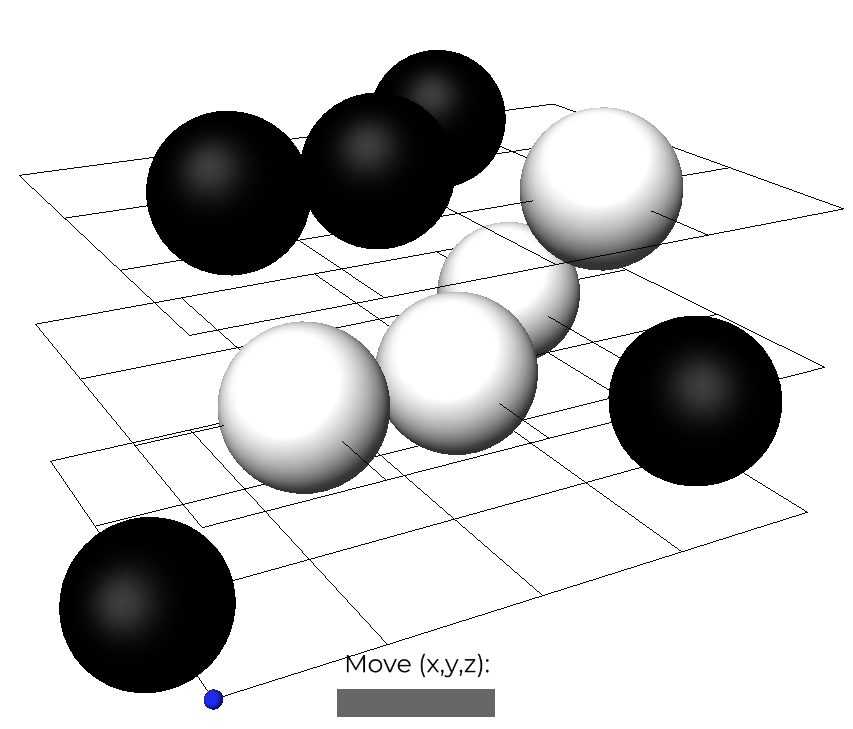
\includegraphics[width=0.5\linewidth]{figures/3dgofoto1}
	\end{center}
	\caption{Go board of size $5\times 4\times 3$ in \href{https://github.com/10500x/3dGo}{3dGo}.}
\end{figure}
Once the rules, arbitrary board-size selection, and other options were implemented, my opponent and I noticed that it was not the same game. \textit{3dGo} felt freer, more aggressive. In our (informal) experience, the greater number of adjacencies altered the playing style, differentiating it from conventional Go. To understand this difference, even without prior experience, we shall analyze the behavior of the average number of adjacencies in the limit\footnote{This was the motivation for initiating this writing.}: Let us examine the limits of the average adjacencies for two- and three-dimensional boards.
\begin{align*}
	\lim_{x,y\to\infty} \tilde{A}(x,y) &= \lim_{x,y\to\infty} \frac{4xy-2x-2y}{xy} = \lim_{x,y\to\infty} \left( 4 - \frac{2x}{xy} - \frac{2y}{xy} \right) = 4,
\end{align*}
\begin{align*}
	\lim_{x,y,z\to\infty} 
	\tilde{A}(x,y,z)&=\lim_{x,y,z\to\infty}\frac{6 x y z - 2 x y - 2 x z - 2 y z}{xyz}=6.\\
\end{align*}
It is evident that the average number of adjacencies in \(\mathrm{Go}^{3}\) is considerably higher. This difference is perceptible in the gameplay experience. The following problem then arises: How can we bring this average closer to $4$? The natural target is a board whose local structure resembles that of \(\mathrm{Go}^{2}\): the aim is a game that imitates Go in rules, size, and gameplay feel, since playing \(\mathrm{Go}^{3}\) as it stands is not playing \(\mathrm{Go}^{2}\). Mean degree is, of course, only a first proxy for how a board plays: two boards with the same mean can have very different degree distributions. We use it as a necessary criterion, not a sufficient one.

\subsection{Removing Nodes, Yes. But How?}
\label{def_partial}

As we have seen, the majority of the nodes on a \(\mathrm{Go}^{3}\) board lie in the interior, provided the size is sufficiently large, where each possesses $6$ adjacencies. Therefore, the elimination of nodes must begin in this region. Next in priority are the faces ($5$ adjacencies), whereas the edges and vertices, possessing $4$ or fewer, do not affect the average we seek. If we consider only the exterior of the board, the faces possess precisely $4$ adjacencies (we lose the one pointing inward); consequently, analyzing their limit, we find that:
\begin{align*}
	\lim_{x,y,z\to\infty} \tilde{A}(x,y,z)_{\partial}&=
	\lim_{x,y,z\to\infty}\frac{8 (x y + x z - 2 x + y z - 2 y - 2 z + 3)}{(xyz)-(x-2)(y-2)(z-2)}=4.
\end{align*}
Thus, our exterior board possesses the same average adjacencies in the limit as \(\mathrm{Go}^{2}\),
$$\lim_{x,y\to\infty}  \tilde{A}(x,y)= \lim_{x,y,z\to\infty} \tilde{A}(x,y,z)_{\partial}.$$
\textit{Remark.} The limit is not really needed to see why. The graph \((G',\sim_{ort}|_{G'})\) is the surface of a box: a $2$-sphere tiled by unit squares. Every face point and every edge point has exactly $4$ adjacencies, exactly as in the interior of $\mathrm{Go}^{2}$, and the only exceptions are the eight corners, which have $3$. Hence
$$A(x,y,z)_{\partial}=4|G'|-8,\qquad \tilde{A}(x,y,z)_{\partial}=4-\frac{8}{|G'|},\qquad |G'|=xyz-(x-2)(y-2)(z-2),$$
which has the same shape as the planar formula \(\tilde{A}(x,y)=4-\tfrac{2(x+y)}{xy}\)


\subsection{Toroidal Board}
\label{key:sectoro}
In \(\mathrm{Go}^{2}\), the limit of the average as the board is made arbitrarily large is $4$. One might ask: is it possible to establish a board whose average liberties are precisely $4$?

If we join the opposite edges of the board, we obtain the following, as shown in Figure~\ref{fig:plano_toro1}.

%\begin{wrapfigure}{i}{0.6\textwidth}
\begin{figure}[H]
	\begin{center}
		\begin{tikzpicture}[scale=1.4]
			
			% Step 1: Plane (square)
			\draw[thick] (0,0) rectangle (2,2);
			\fill[color=sealred] (0,2) circle (0.05);
			\fill[color=sealred] (0,0) circle (0.05);
			\fill[color=bg] (2,0) circle (0.05);
			\fill[color=bg] (2,2) circle (0.05);
			
			% Step 2: Cylinder
			\begin{scope}[xshift=3cm]
				
				\draw[thick] (0,0) arc[start angle=-180, end angle=0, radius=0.5cm] -- (1,2) arc[start angle=0, end angle=-180, radius=0.5cm] -- cycle;
				
				
				\draw[black, dashed] (1,1) arc[start angle=0, end angle=-180, radius=0.5cm];
				\fill[color=sealred] (0,0) circle (0.05);
				\fill[color=bg] (1,0) circle (0.05);
				\fill[color=sealred] (0,2) circle (0.05);
				\fill[color=bg] (1,2) circle (0.05);
			\end{scope}
			
			\begin{scope}[xshift=5cm]
				\draw[thick] (0,0) arc[start angle=180, end angle=0, radius=0.25cm] -- (.5,2) arc[start angle=0, end angle=180, radius=0.25cm] -- cycle;
				\draw[thick] (0,0) arc[start angle=-180, end angle=0, radius=0.25cm] -- (0.5,2) arc[start angle=0, end angle=-180, radius=0.25cm] -- cycle;
				\fill[color=sealred!50!bg] (0,2) circle (0.05);
				\fill[color=sealred!50!bg] (0,0) circle (0.05);
				\draw[black, dashed] (0.5,1) arc[start angle=0, end angle=360, radius=0.25cm];
				
			\end{scope}
		\end{tikzpicture}
	\end{center}
	\caption{Transition from the plane to a cylinder by joining its opposite sides.}
	\label{fig:plano_toro1}
\end{figure}

Let us repeat the process; let us join our $4$ vertices—which are now $2$—into a single one, Figure~\ref{fig:plano_toro2}.

%\begin{wrapfigure}[15]{r}{0.57\textwidth}
\begin{figure}[H]
	\begin{center}   
		\begin{tikzpicture}[scale=1.4]
			
			%% Cilindro base
			\draw[thick] (0,0) arc[start angle=180, end angle=0, radius=0.25cm] -- (.5,2) arc[start angle=0, end angle=180, radius=0.25cm] -- cycle;
			\draw[thick] (0,0) arc[start angle=-180, end angle=0, radius=0.25cm] -- (0.5,2) arc[start angle=0, end angle=-180, radius=0.25cm] -- cycle;
			\fill[color=sealred!50!bg] (0,2) circle (0.05);
			\fill[color=sealred!50!bg] (0,0) circle (0.05);  
			%\draw[black, dashed] (0.5,1) arc[start angle=0, end angle=360, radius=0.25cm];
			
			
			
			%% Cilindro semi transición
			\begin{scope}[xshift=1.5cm]
				%% Cuerpo de cilindro
				\draw[thick] (0,1.5) -- (0,0.5);
				\draw[thick] (0.5,1.5) -- (0.5,0.5);
				\draw[thick, dashed] (0.75,1.5) -- (0.75,0.5);
				\draw[thick, dashed] (1.25,1.5) -- (1.25,0.5);
				\draw[black, dashed] (1.25,1) arc[start angle=0, end angle=360, radius=0.25cm];
				%%Arcos superiores
				\draw[thick] (0.5,1.5) arc[start angle=180, end angle=0, radius=0.125cm] ;
				\draw[thick](1.25,1.5) arc[start angle=0, end angle=180, radius=0.625cm];
				
				%%Arcos inferiores
				\draw[thick] (0,0.5) arc[start angle=-180, end angle=0, radius=0.625cm] ;
				\draw[thick] (0.5,0.5) arc[start angle=-180, end angle=0, radius=0.125cm] ;
				
				\fill[color=sealred!50!bg] (1.25,1.5) circle (0.05);
				\fill[color=sealred!50!bg] (1.25,0.5) circle (0.05);
				
			\end{scope}
			
			%% Toro
			\begin{scope}[xshift=3.75cm]
				
				%%Circulo externo
				\draw[thick] (0,1) arc[start angle=180, end angle=-180, radius=1cm];
				%%Cirulo interno
				\draw[thick] (0.5,1) arc[start angle=180, end angle=-180, radius=0.5cm];
				%Aristas
				\draw[black, dashed] (2,1) arc[start angle=0, end angle=360, radius=0.25cm];
				%% vértices / vértice
				\fill[color=sealred!50!bg] (2,1) circle (0.05);
				
			\end{scope}
		\end{tikzpicture}
	\end{center}
	\caption{Transition from the cylinder to the torus after joining its opposite faces.}
	\label{fig:plano_toro2}
\end{figure}
Let us observe how the adjacencies of the vertices have changed: in the plane, we saw that they were $2$ for each, but in the cylinder, it can be seen that they have $3$, and furthermore, on the torus, they are $4$. The same occurs with the nodes on the edges, Figure~\ref{fig:Fig 27}.
%\begin{wrapfigure}{r}{0.6\textwidth}
\begin{figure}[H]
	\begin{center}
		\begin{tikzpicture}[scale=1.4]
			
			% Plano 
			\draw[thick] (0,0) rectangle (2,2);
			
			
			%Libertades nodo rojo
			\draw[YellowOrange, ultra thick] (0,2) -- (0.25,2); %Derecha
			\draw[YellowOrange, ultra thick] (0,2) -- (0,1.75); %Derecha
			%Libertades nodo verde
			\draw[YellowOrange, ultra thick] (2,1) -- (2,1.25);
			\draw[YellowOrange, ultra thick] (2,1) -- (2,0.75);
			\draw[YellowOrange, ultra thick] (2,1) -- (1.75,1);
			
			%nodos
			\fill[color=Moss] (2,1) circle (0.05);
			\fill[color=sealred] (0,2) circle (0.05);
			\fill[color=sealred] (0,0) circle (0.05);
			\fill[color=bg] (2,0) circle (0.05);
			\fill[color=bg] (2,2) circle (0.05);
			
			
			
			
			%% Cilindro 
			\begin{scope}[xshift=3cm]
				
				\draw[thick] (0,0) arc[start angle=180, end angle=0, radius=0.25cm] -- (.5,2) arc[start angle=0, end angle=180, radius=0.25cm] -- cycle;
				\draw[thick] (0,0) arc[start angle=-180, end angle=0, radius=0.25cm] -- (0.5,2) arc[start angle=0, end angle=-180, radius=0.25cm] -- cycle;
				
				
				
				
				%%% vértices Aristas cilindro
				\draw[YellowOrange, ultra thick] (0,2) arc[start angle=-180, end angle=-115, radius=0.25cm];
				\draw[YellowOrange, ultra thick] (0,2) arc[start angle=180, end angle=115, radius=0.25cm];
				\draw[YellowOrange, ultra thick] (0,2) -- (0,1.60); %Abajo
				
				%%% Naranja, libertades y linea punteada
				\draw[YellowOrange, ultra thick] (0.5,1) -- (0.5,1.25);
				\draw[YellowOrange, ultra thick] (0.5,1) -- (0.5,0.75);
				\draw[black, dashed] (0.5,1) arc[start angle=0, end angle=360, radius=0.25cm];
				\draw[YellowOrange, ultra thick] (0.5,1) arc[start angle=0, end angle=70, radius=0.25cm];
				\draw[YellowOrange, ultra thick] (0.5,1) arc[start angle=0, end angle=-70, radius=0.25cm];
				
				%%%% vértices
				\fill[color=sealred!50!bg] (0,2) circle (0.05);
				\fill[color=sealred!50!bg] (0,0) circle (0.05);
				\fill[color=Moss] (0.5,1) circle (0.05);
			\end{scope}
			
			
			%% Toro
			\begin{scope}[xshift=4.5cm]
				%%Circulo externo
				\draw[thick] (0,1) arc[start angle=180, end angle=-180, radius=1cm];
				%%Cirulo interno
				\draw[thick] (0.5,1) arc[start angle=180, end angle=-180, radius=0.5cm];
				
				
				
				%%% Aristas nodo  morado
				\draw[YellowOrange, ultra thick] (2,1) arc[start angle=0, end angle=15, radius=1cm];
				\draw[YellowOrange, ultra thick] (2,1) arc[start angle=0, end angle=-15, radius=1cm];
				\draw[black, dashed] (2,1) arc[start angle=0, end angle=360, radius=0.25cm];
				\draw[YellowOrange, ultra thick] (2,1) arc[start angle=0, end angle=70, radius=0.25cm];
				\draw[YellowOrange, ultra thick] (2,1) arc[start angle=0, end angle=-70, radius=0.25cm];
				
				%% vértices
				\fill[color=sealred!50!bg] (2,1) circle (0.05);
				\fill[Moss] (1.5,1) circle (0.05);
			\end{scope}
			
		\end{tikzpicture}
	\end{center}
	\caption{Change in adjacencies from the plane to the torus.}
	\label{fig:Fig 27} % Assign a unique label
\end{figure}
It is therefore worth asking: Is it possible to do this in any dimension? That is, taking them to their ``toroidal'' form. Indeed, it is possible, and furthermore, it is very simple and, unlike Figure~\ref{fig:Fig 27}, we do not lose points.

Under our scrutiny, $G$ contains only points, and the adjacency criterion determines their relationships. To relate the edges, it suffices to add new relationships. What we seek is to join each face with its opposite; to achieve this, we formulate the following definition of the adjacency criterion by opposites, denoted as \(\sim_{op}\). Let \(G = N_1 \times \dots \times N_n\) be an $n$-dimensional board, where \(|N_k| = n_k \ge 3\). We shall say that two points $g_1, g_2 \in G$ are oppositely related if they are identical in all their coordinates except in one, the $k$-th, where they take values at the extremes:
\begin{equation*}
	g_1=(x_1,\dots, 1, \dots, x_n) \ \sim \ (x_1, \dots, n_k, \dots, x_n)=g_2.
\end{equation*}
Thus, in this simple manner, we have defined the toroidal board, which is nothing more than the same board as before, except that we are now considering more adjacent points. Formally, if we call the canonical criterion \(\sim_{\text{ort}}\) (orthogonal adjacencies), we transition from the form \((G,\sim_{\text{ort}})\) to $(G, \sim_{\text{ort}} \cup \sim_{\text{op}})$.

It is clear that the toroidal board will have $4$ adjacencies for each of its nodes. Let \(A(x,y)_{T}\) be the number of adjacencies on a toroidal board of size \(xy\); let us carry out once again the process we performed at the beginning. The toroidal board will have no vertices, no edges, and consequently, a single face composed of \(xy\) nodes which, as we have already seen, possess $4$ adjacencies per node; thus:
$$A(x,y)_{T}=4xy.$$
And its average will be $4$, since:
$$\tilde{A}(x,y)_{T}=4xy/xy=4.$$
In this way, we have found a board such that for every node, the number of adjacencies is uniform. Let us do the same in $\mathrm{Go}^{3}$; we can formulate the following scheme from Figure~\ref{carasgo3}.

Here, if we apply the new relation, we obtain that all points will have $6$ adjacencies. Indeed, the vertices will acquire $3$ new adjacencies, bringing them to $6$; the edges will acquire $2$ new adjacencies, bringing them to $6$; and finally, the faces will acquire a single new adjacency—the opposite one. Thus, equality is achieved in the limit.
\begin{figure}[H]
	\centering
	\begin{tikzpicture}[scale=1]
		\pgfmathsetmacro{\x}{-5}
		\pgfmathsetmacro{\y}{6}
		\pgfmathsetmacro{\z}{1.5}
		
		
		%nodo que está atrás
		\fill[color=terracotta] (-5,0) circle (0.07);
		
		\path (0,0,\y) coordinate (A) (\x,0,\y) coordinate (B) (\x,0,0) coordinate (C) (0,0,0)
		coordinate (D) (0,\z,\y) coordinate (E) (\x,\z,\y) coordinate (F) (\x,\z,0) coordinate (G)
		(0,\z,0) coordinate (H);
		\draw  (A)-- (B)-- (C)--(G)--(F)-- (B) (A)--(E)--(F)--(G)--(H)--(E);
		\draw [dashed,black] (A)--(D)-- (C)-- (D)--(H);
		
		%nodo y sus aristas
		
		
		\draw (-2.5,0.75) node [thick,scale=2]{$A$};
		\draw (-4.85,-1.55) node [thick,scale=2]{$A'$};
		
		
		
		\draw (-1.15,-0.45) node [thick,scale=2,rotate=0,yslant=1,xslant=-0.25]{$B$};
		\draw (-6,-0.25) node [thick,scale=2,rotate=0,yslant=1,xslant=-0.25]{$B'$};
		
		\draw (-3.5,-1.15) node [thick,scale=2,yslant=0,xslant=0.75]{$C$};
		\draw (-3.5,0.35) node [thick,scale=2,xslant=0.75]{$C'$};
		
		\fill[color=terracotta] (-5,1.5) circle (0.07);
		\fill[color=terracotta] (0,0) circle (0.07);
		\fill[color=terracotta] (0,1.5) circle (0.07);
		
		
		\fill[color=sealred] (-7.3,-2.3) circle (0.07);
		\fill[color=sealred] (-7.3,-0.8) circle (0.07);
		\fill[color=sealred] (-2.3,-0.8) circle (0.07);
		\fill[color=sealred] (-2.3,-2.3) circle (0.07);
		
	\end{tikzpicture}
	\caption{Faces of the $\mathrm{Go}^{3}$.}
	\label{carasgo3}
\end{figure}

Now then, what would happen if we consider only the points lying on the boundary?

If \(x\in G\), \(x=(x_1,\dots,x_n)\) with \(x_i \leq n_i = |N_i|\), the boundary will be that of the points given by
$$G'=\{x\in G: \exists i, (x_i= 1 \lor x_i =n_i) \}.$$ Through the canonical adjacency criterion, we obtain a board such that it possesses, in the limit, $4$ adjacencies per point, since only the vertices possess $3$ adjacencies, as we saw in Section~\ref{def_partial}.

If we attach to this board the adjacencies given by the opposite criterion, obtaining \((G',\sim_{\text{ort}} \cup \sim_{\text{op}})\), it will have $5$ adjacencies for every face point (and $6$ for edge and vertex points); since they lack the interior points, the faces lose one adjacency, but they gain it back through the opposite face. The edges, which possess $4$ adjacencies, gain $2$, and the vertices obtain $3$. Since the faces account for the largest number of points, it is clear that their limit will be $5$, naturally, when scaled to large sizes.

If we recall Lemma~\ref{lem:2n}, upon applying these procedures to any given board, we can always achieve the equality of $2n$ adjacencies per point, for the opposite criterion guarantees the filling of all missing adjacencies. It is easy to see that, by taking arbitrarily large boards, any \(n\)-dimensional board possesses an average of $2n$ adjacencies in the limit.

For this problem, for \(n=2\), \(\sim_{ort}\) provides a solution for the case with a degree as close to $4$ as possible, whereas the relation \( \sim_{ort} \cup \sim_{{op}}\) satisfies the degree condition of exactly $4$. Furthermore, for the case \(n = 3\), we were able to find a partial solution on the boundary: if \(G' = \{ x \in G \mid \exists i \text{ such that } (x_i = 1 \lor x_i = n_i) \}\) denotes the boundary, then the graph \((G', \sim_{ort}|_{G'})\) is a solution for the case with a degree as close to $4$ as possible on the surface.

\section{Go in One Dimension}\label{Go_1dim}
%\begin{figure}[H]
\begin{wrapfigure}[5]{r}{0.4\textwidth}
	\centering
	\begin{goban}[7x1]
		\pgfgoticks
	\end{goban}
	
	\medskip
	
	\begin{goban}[7x1]
		\pgfgoticks
		\moves{E1, C1}
	\end{goban}
	\caption{Empty board and board with a black and a white stone.}
	\label{fig:1dim_go}
\end{wrapfigure}
First, let us examine what it looks like, Figure~\ref{fig:1dim_go}. Clearly, there are two liberties per point, except at the boundaries, which possess one. Therefore,
\begin{align*}
	A(n)&=2\cdot 1+(n-2)\cdot 2=2n-2.\\
	\tilde{A}(n)&=\frac{2n-2}{n}=2-\frac{2}{n}.
\end{align*}
Then, it is clear that the limit of its average is $2$.

\label{teoremas_go1}
\begin{lemma}
	In canonical $\mathrm{Go}^1$ on $G = \{1, \dots, n\}$ ($n \ge 3$), the only
	vacant regions $R \in I^0$ (i.e., $e$-regions with $R = R_0$) that can constitute
	an eye are the single-point extreme regions $(0,1)$ and $(0,n)$. Any
	other interior vacant vital region is necessarily a single-point joiner.
\end{lemma}
\begin{proof}
	Every connected empty region $R$ corresponds to a discrete interval of vacant points $P(R) = \{a, a+1, \dots, b\}$ with $1 \le a \le b \le n$.
	\begin{figure}[H]
		\centering
		\begin{goban}[7x1]
			\pgfgoticks
			\stones[b]{D1, F1}
			\stone[w]{B1}
			\mark[filled square, fill = {true, color = amethyst}, line = {color = black}]{A1}
			\mark[filled square, fill = {true, color = bg}, line = {color = black}]{E1}
		\end{goban}
		\caption{\textcolor{amethyst}{Eye} at the boundary, \textcolor{bg}{joiner} in the interior.}
		\label{fig:ej_go1dim}
	\end{figure}
	\begin{itemize}
		\item \textbf{$R$ in the interior ($1 < a \le b < n$):} The adjacency set of $R$ consists of the
		stones at $a-1$ and $b+1$.
		Since the interval $\{a, \dots, b\}$ is vacant, no path of stones of
		color $e \neq 0$ can connect $a-1$ to $b+1$. Thus, the stones $(e, a-1)$ and $(e, b+1)$ belong
		to two distinct groups $I_1 \neq I_2$, so $|\partial R| = 2$.
		Consequently, $R$ cannot be an eye; if $b = a$ and $I_1, I_2 \in P$ share color $e$, $R = \{(0, a)\}$ is a joiner.
		
		\item \textbf{$R$ at the boundary ($a = 1$ or $b = n$):} Suppose $a = 1$ (the case $b = n$ is
		analogous). If $b = n$, the board is empty.
		If $b < n$, the only stone adjacent to $R$ lies at $b+1$, belonging to a single group $I$ ($|\partial R| = 1$).
		For $R$ to be healthy for $I$ ($R_0 \subseteq L(I)$), every point in $P(R)$ must be adjacent to $b+1$, which forces $a = b = 1$. Hence $R = \{(0, 1)\}$ is an eye for $I$.
	\end{itemize}
\end{proof}
\section{Common Origin}

Thus far, we have constructed two-dimensional Go and explored its generalizations to one and three dimensions. Although their dynamics differ, a natural question arises: are they truly distinct structures? We shall see that all of them can be derived from a single common origin.

\paragraph{What is being varied.} The triple $\Gamma=(G,E,\sim)$ is the \emph{arena} of a game: where it is played, who takes part, and what is next to what. Go is this arena together with the rule schema $\Delta$ of Part~II (placement, capture, suicide, superko). In this section $\Delta$ is held fixed and only the arena varies; in Section~\ref{sec_JR} the rules vary as well.

\paragraph{Axis boards.} The operations below act coordinate by coordinate, and that information is not recorded in the bare triple $(G,E,\sim)$. In particular, the relation $\sim_{op}$ of Section~\ref{key:sectoro} only makes sense once we know which points are ``opposite'', that is, which coordinates are the extremes of which axis. We therefore record it.

\begin{definition}[Axis board]
	An \emph{axis} is a pair $a=(n_a,\kappa_a)$ with $n_a\ge 1$ and $\kappa_a\in\{\mathrm{path},\mathrm{cycle}\}$, where $n_a\ge 3$ if $\kappa_a=\mathrm{cycle}$. An \emph{axis board} $B=(a_1,\dots,a_d;E)$ is a list of $d\ge 0$ axes together with a state set $E\ni 0$. Its structure is $\Gamma(B)=(G,E,\sim)$, where $G=\prod_{i=1}^{d}\{1,\dots,n_{a_i}\}$ and $g\sim h$ if and only if $g$ and $h$ differ in exactly one coordinate $i$, and there $h_i-g_i=\pm1$ if $a_i$ is a path, or $h_i-g_i\equiv\pm1 \pmod{n_{a_i}}$ if $a_i$ is a cycle.
\end{definition}

When every axis is a path, $\sim$ is the orthogonal adjacency $\sim_{ort}$; turning a path of length $n_a\ge3$ into a cycle adds exactly the relation $\sim_{op}$ along that axis. We write $\mathrm{Go}^n_m(n_1,\dots,n_n)$ for the board with $n$ path axes of lengths $n_1,\dots,n_n$ and $E=\{0,1,\dots,m\}$, and $\mathrm{Go}^n_m$ for the family obtained by letting the sizes vary. With no axes, $G$ is a single point; this is $\mathrm{Go}^0_0=(\{\ast\},\{0\},\sim)$, a single-node game with no players.

Four operations act on axis boards.
\begin{itemize}
	\item \textbf{Adding a player,} $\iota$. It replaces $E$ by $E\cup\{y\}$ with $y\notin E$, and leaves the board untouched. It is injective on states ($\iota(e_1)=\iota(e_2)\Rightarrow e_1=e_2$), preserves the identity of the previous states, and is non-surjective so as to accommodate the new element.
	\item \textbf{Adding an axis,} $\Xi_k$. It appends the path axis $M=\{1,\dots,k\}$, so $G$ becomes $G\times M$ with the product adjacency
	$$(g,m)\sim_{G\times M}(g',m')\iff\bigl(g\sim g'\ \text{and}\ m=m'\bigr)\ \text{or}\ \bigl(g=g'\ \text{and}\ |m-m'|=1\bigr).$$
	For every slice $m\in M$ the embedding $\xi_m(g)=(g,m)$ is injective and satisfies $\xi_m(g_1)\sim\xi_m(g_2)\iff g_1\sim g_2$. For $k=1$ this is the plain embedding $g\mapsto(g,1)$, which raises the dimension without changing the board.
	\item \textbf{Wrapping axes,} $\tau_S$ for $S\subseteq\{1,\dots,d\}$. It turns the axes in $S$ into cycles (each of length $\ge3$), and is the identity on $G$ and $E$. In terms of $\Gamma$, it replaces $\sim$ by $\sim\cup\sim^{S}_{op}$; hence $g_1\sim g_2\Rightarrow\tau_S(g_1)\sim\tau_S(g_2)$, and $\tau_S$ is an injective, adjacency-preserving map. We write $\tau=\tau_{\{1,\dots,d\}}$ for the operation that wraps \emph{every} axis.
	\item \textbf{Adding a cyclic axis,} $\Xi^{cyc}_k:=\tau_{\{d+1\}}\circ\Xi_k$ for $k\ge3$.
\end{itemize}

\begin{lemma}[Commutation]\label{lem:conmutacion}
	Let $B$ be an axis board with $d$ axes.
	\begin{enumerate}
		\item $\iota$ commutes with $\Xi_k$ and with every $\tau_S$.
		\item $\tau_S\circ\Xi_k=\Xi_k\circ\tau_S$ for every $S\subseteq\{1,\dots,d\}$.
		\item $\tau\circ\Xi_k=\Xi^{cyc}_k\circ\tau$ (for $k\ge3$), where $\tau$ wraps every axis of the board it is applied to.
		\item In general $\tau\circ\Xi_k\neq\Xi_k\circ\tau$: on the left the new axis is a cycle, on the right it is a path.
	\end{enumerate}
\end{lemma}
\begin{proof}
	Each operation acts on a different part of the data (the list of axes, or $E$), or on different entries of that list: $\iota$ changes $E$, $\Xi_k$ appends an entry, and $\tau_S$ changes the type of the entries in $S$. Operations acting on different parts commute, which gives (1) and (2). For (3), both sides produce the board whose first $d$ axes are cycles and whose new axis is a cycle of length $k$. For (4), the left side wraps the new axis, while on the right $\tau$ has already acted before the axis was appended. \end{proof}

Fixing the sizes at each step, the operations $\iota$ and $\Xi$ organize the games into the following family (Figure~\ref{fig:familia-go}).
\begin{figure}[H]
	\centering
	\begin{tikzcd}
		{Go_0^0} && {Go_1^0} && {Go_m^0} \\
		\\
		{Go_0^1} && {Go_1^1} && {Go_m^1} \\
		\\
		{Go_0^n} && {Go_1^n} && {Go_m^n}
		\arrow["id"{description}, from=1-1, to=1-1, loop, in=215, out=145, distance=10mm]
		\arrow["\iota", hook, from=1-1, to=1-3]
		\arrow["\Xi", hook, from=1-1, to=3-1]
		\arrow[dashed, from=1-1, to=3-3]
		\arrow["\dots", hook, from=1-3, to=1-5]
		\arrow["\Xi", hook, from=1-3, to=3-3]
		\arrow["\Xi", hook, from=1-5, to=3-5]
		\arrow["\iota", hook, from=3-1, to=3-3]
		\arrow["\vdots", hook, from=3-1, to=5-1]
		\arrow["\dots", hook, from=3-3, to=3-5]
		\arrow["\vdots", hook, from=3-3, to=5-3]
		\arrow[dashed, from=3-3, to=5-5]
		\arrow["\vdots", hook, from=3-5, to=5-5]
		\arrow["\iota"', hook, from=5-1, to=5-3]
		\arrow["\dots"', hook, from=5-3, to=5-5]
	\end{tikzcd}
	\caption{Structure of the family of \textit{Go Games}. Players are added to the right ($\iota$); axes are appended downward ($\Xi_k$, with the size $k$ chosen at each step). Starting from the single point $\mathrm{Go}^0_0$, appending one axis of length $k$ gives a line of $k$ points.}
	\label{fig:familia-go}
\end{figure}
Recalling 老子 — \textit{Laozi}, we rediscover what has already been stated:\\
\noindent
\begin{minipage}[t]{0.35\textwidth}
	\begin{flushright}
		{\large
			\vspace{1pt}
			道生一，\\
			一生二，\\
			二生三，\\
			三生万物。
		}
	\end{flushright}
\end{minipage}%
\hfill
\vrule
\hfill
\begin{minipage}[t]{0.48\textwidth}
	\raggedright
	\vspace{1pt}
	\emph{
		$\ \!\!\!$The way brings forth one, \\
		One brings forth two, \\
		Two brings forth three, \\
		Three brings forth all things.}
\end{minipage}

\vspace{1pt}
\hfill  道德經 — {\textsc{Dàodé jīng Chapter 42}}\\

\paragraph{The toroidal family.} By Section~\ref{key:sectoro}, wrapping every axis of a board with all sizes $\ge3$ gives a board in which every point has the same number of adjacencies, $2d$. We write $\mathrm{T}^n_m:=\tau(\mathrm{Go}^n_m)$. The mapping $\tau$ alters neither the number of nodes nor the players; it only adds relations between opposite positions. By Lemma~\ref{lem:conmutacion}, the square of Figure~\ref{fig:hollow_torus} commutes as soon as the expansion on the torus row is the cyclic one, $\Xi^{cyc}$.

\paragraph{The hollow torus.} On the other hand, recalling the adjacency analysis of Section~\ref{chap:6}, boundary positions behave differently from interior ones. To isolate this phenomenon we introduce the boundary restriction operator
$$\partial:(G,E,\sim)\to(\partial G,E,\sim|_{\partial G}),$$
where $\partial G=\{x\in G:\exists i,\ x_i=1\ \text{or}\ x_i=n_i\}$ and $\sim|_{\partial G}=\sim\cap(\partial G\times\partial G)$ is the induced relation, as in Section~\ref{key:sectoro}. Its output is a general structure and no longer an axis board, so $\partial$ can only be applied last. Moreover, on a cyclic axis the ``extremes'' $1$ and $n_i$ depend on where the cycle was cut, so $\partial$ of a torus is defined relative to the chosen coordinates.

The operator $\partial$ does not commute with $\Xi_k$, since the boundary of a Cartesian product obeys the geometric Leibniz rule
\[
\partial(G \times M) = (\partial G \times M) \cup (G \times \partial M) \neq \partial G \times M.
\]
Consequently, hollowing out the interior must be performed after expanding the dimensions of the board (with $d\ge2$ axes of length $\ge3$). Combining the operators gives the diagram of Figure~\ref{fig:hollow_torus}: $\Xi$ and $\iota$ commute with $\tau$ (using $\Xi^{cyc}$ on the torus row) to generate the toroidal family $\mathrm{T}^n_m$, followed by the boundary restriction $\partial$ onto the hollow torus $\partial\mathrm{T}^n_m$.
\begin{figure}[ht]
	\centering
	\begin{tikzcd}
		{Go_{0}^{0}} &&& {Go_{m}^{n}} && \\
		\\
		\\
		{T_{0}^{0}} &&& {T_{m}^{n}} && {\partial T_{m}^{n}}
		\arrow["{\Xi , \iota}"{description}, hook, from=1-1, to=1-4]
		\arrow["\tau"{description}, maps to, from=1-1, to=4-1]
		\arrow[dashed, from=1-1, to=4-4]
		\arrow["\tau"{description}, maps to, from=1-4, to=4-4]
		\arrow["{\Xi^{cyc} , \iota}"{description}, hook, from=4-1, to=4-4]
		\arrow["\partial"{description}, from=4-4, to=4-6]
	\end{tikzcd}
	\caption{Diagram of the complete structure. The horizontal arrows expand dimensions and players ($\Xi$ on paths, $\Xi^{cyc}$ on cycles, $\iota$), $\tau$ closes the board into a torus, and $\partial$ hollows out the interior.}
	\label{fig:hollow_torus}
\end{figure}

\paragraph{The projection onto the graph.} To study the geometric properties of the board, as in Section~\ref{chap:6}, it is useful to temporarily ignore the state of the positions and the game dynamics. We thus define the mapping
\[U:(G,E,\sim)\to (G,\sim).\]
This mapping associates each game with its underlying graph. In this way, properties such as the number of adjacencies $A(x,y)$ can be studied solely from the adjacency structure. Note that different games may determine the same graph, so the mapping is not injective.

\newpage

\section{Toward Surrounding Games}\label{sec_JR}

Let us see how our theory could take us further than we initially thought. A caveat first: besides the arena $\Gamma=(G,E,\sim)$, each game below needs three more ingredients, which we make explicit: a family $\mathcal{D}$ of distinguished subsets of $G$ (corners, edges, the incidence sets of Shannon's game), a rule schema $\Delta$, and a winning condition $W$ phrased in terms of groups, regions and the sets in $\mathcal{D}$. A \emph{surrounding game} is thus a tuple $(\Gamma,\mathcal{D},\Delta,W)$; Go itself has $\mathcal{D}=\varnothing$ and the rules of Part~II. What the examples show is that the arena, together with the notions of group, region and liberty, is enough to state $W$ in each case.

\subsection*{Othello}

\begin{wrapfigure}[13]{i}{0.35\textwidth}
	
	\centering
	\begin{goban}
		[goban={
			size=9,
			scale=1.25,
			background ={
				fill = {color = othello},
				line = {color = othelloborder}},
			hoshi = {false}
		}]
	\end{goban}
	\caption{Othello board.}
	\label{fig:Tab_Othello}
\end{wrapfigure}In Figure~\ref{fig:Tab_Othello}, on the Othello board, play takes place inside the squares; this poses no difficulty, as it suffices to think of the intersections as the squares. Unlike Go, stones are adjacent in all directions (diagonals too); we simply need to modify \(\sim\). Furthermore, in Othello, ``capturing'' consists of flipping the stones to change their color. In turn, to ``surround,'' it is only necessary to do so in one dimension, that is, to enclose a group of another color along a straight line, either orthogonally or diagonally. We can already accomplish this: it suffices to consider that upon capturing, instead of removing the stones (i.e., assigning \(C(i)=0\)), we assign the color of the capturing player (by flipping them). If we had \(\Delta_{Oth}\), Othello can be constructed over the game:
$(N\times N, \{0,1,2\}, \sim_{ort} \cup \sim_{diag}).$	With $|N|=8$, $\sim_{diag}$ being the criterion that takes diagonals $(\pm1,\pm1)$ into account, and $\Delta_{Oth}$ the rules of change in Othello. Note that here the framework supplies only the arena: ``surrounding'' is a condition along straight lines, not on groups, so the capture mechanism lives entirely in $\Delta_{Oth}$. The construction suggests a possible formalization of \textit{Othello} within the same framework, but a weaker one than for Go.

\newpage


\subsection*{Havannah}

\begin{wrapfigure}[13]{r}{0.35\textwidth}
	\vspace{-10pt}
	\centering
	\begin{tikzpicture}[scale=0.55] \tikzstyle{every node}=[font=\small]
		
		% Parámetros del hexágono
		\def\r{0.58}
		
		% Función para dibujar una celda hexagonal
		\foreach \q in {-4,...,4}{
			\pgfmathtruncatemacro{\rmin}{max(-4,-\q-4)}
			\pgfmathtruncatemacro{\rmax}{min(4,-\q+4)}
			\foreach \s in {\rmin,...,\rmax}{
				\pgfmathsetmacro{\x}{0.575*sqrt(3)*(\q+\s/2)}
				\pgfmathsetmacro{\y}{0.575*1.5*\s}
				
				\draw[fill=goban]
				(\x,\y)
				++(30:\r)
				\foreach \a in {90,150,210,270,330}{
					-- ++(\a:\r)
				} -- cycle;
			}
		}
		
		% ------------------------
		% Anillo (azul)
		% ------------------------
		
		\foreach \q/\s in {
			0/1,1/0,1/-1,0/-1,-1/0,-1/1, -1/1
		}{
			\pgfmathsetmacro{\x}{0.575*sqrt(3)*(\q+\s/2)}
			\pgfmathsetmacro{\y}{0.575*1.5*\s}
			
			\filldraw[fill=bg]
			(\x,\y)
			++(30:\r)
			\foreach \a in {90,150,210,270,330}
			{ -- ++(\a:\r) } -- cycle;
		}
		
		% ------------------------
		% Puente (rojo)
		% ------------------------
		
		\foreach \q/\s in {
			-4/0, 	-3/0, -3/1,-3/2,-3/3,-4/4
		}{
			\pgfmathsetmacro{\x}{0.575*sqrt(3)*(\q+\s/2)}
			\pgfmathsetmacro{\y}{0.575*1.5*\s}
			
			\filldraw[fill=sealred]
			(\x,\y)
			++(30:\r)
			\foreach \a in {90,150,210,270,330}
			{ -- ++(\a:\r) } -- cycle;
		}
		
		% ------------------------
		% Tenedor (verde)
		% ------------------------
		
		\foreach \q/\s in {
			1/-2, 2/-2,3/-2, 3/-2, 
			1/-3, 1/-4,
			3/-1, 4/-2, 3/0, 3/1
		}{
			\pgfmathsetmacro{\x}{0.575*sqrt(3)*(\q+\s/2)}
			\pgfmathsetmacro{\y}{0.575*1.5*\s}
			
			\filldraw[fill=Moss]
			(\x,\y)
			++(30:\r)
			\foreach \a in {90,150,210,270,330}
			{ -- ++(\a:\r) } -- cycle;
		}
	\end{tikzpicture}
	\caption{The three winning structures in Havannah: \textcolor{bg}{ring}, \textcolor{sealred}{bridge}, and \textcolor{Moss}{fork}.}
	\label{fig:havannah}
\end{wrapfigure}
Another interesting example is Havannah. Unlike Go, this game takes place on a hexagonal board, and stones are adjacent according to the intrinsic geometry of said board. Once again, it suffices to modify the adjacency criterion. The particularity of Havannah is that there are three distinct ways to win: constructing a \textcolor{bg}{ring}, a \textcolor{sealred}{bridge}, or a \textcolor{Moss}{fork} (see Figure~\ref{fig:havannah}).

Our theory already accounts for the case of the ring: a group $I \in I^e(T)$
forms a ring if it encloses a non-empty component $X \subseteq \text{Interior}$
($\mathcal{K}(X) \subseteq I$).\footnote{Unlike an eye in Go, a ring in Havannah
	cannot use the board perimeter as part of its boundary, which is why the
	enclosed cells must lie in $\text{Interior}$; those cells may be vacant or
	occupied.} If we distinguish the six corners and the six sides of the board via
the degree $|\mathcal{K}(i)|$ (Section 2.1):
\begin{itemize}
	\item $\text{Corners} = \{i \in T : |\mathcal{K}(i)| = 3\}$ (six isolated
	corner positions),
	\item $\text{Edges} = \{i \in T : |\mathcal{K}(i)| = 4\}$ (whose six
	connected components $E_1, \dots, E_6$ are the six sides of the board),
	\item $\text{Interior} = \{i \in T : |\mathcal{K}(i)| = 6\}$,
\end{itemize}
setting $\mathcal{D} = \{\text{Corners}, E_1, \dots, E_6, \text{Interior}\}$
allows us to express all three winning conditions: a \emph{bridge} is a group
$I$ with $|I \cap \text{Corners}| \ge 2$, and a \emph{fork} is a group $I$
intersecting at least three distinct sides $E_m$.
In this manner, Havannah's winning condition can be expressed solely in terms of groups, regions, and board subsets. Consequently, the game appears to admit a natural formalization within the same theoretical framework. 

\subsection*{Hex}
\begin{wrapfigure}[12]{i}{0.47\textwidth}
	\centering
	\begin{tikzpicture}[scale=0.4]
		\def\r{0.55}
		
		%% Borde de colores de cada jugador
		\coordinate (TL) at (4.2,9.7);
		\coordinate (TR)at (16,9.7);
		\coordinate (BL) at (-1.5,-0.35);
		\coordinate (BR) at (10,-0.35);
		\coordinate (C) at (7,5);
		
		\fill[bg] (TL) -- (C) -- (TR) -- cycle;
		\fill[bg] (BL) -- (C) -- (BR) -- cycle;
		
		\fill[sealred] (TL) -- (C) -- (BL) -- cycle;
		\fill[sealred] (TR) -- (C) -- (BR) -- cycle;
		\draw[thick] (TL)--(TR)--(BR)--(BL)--cycle;
		
		
		% Tablero 11x11 tipo Hex
		\foreach \i in {0,...,10}{
			\foreach \j in {0,...,10}{
				
				\pgfmathsetmacro{\x}{0.55*sqrt(3)*(\i+\j/2)}
				\pgfmathsetmacro{\y}{0.55*1.5*\j}
				
				\draw[fill=goban]
				(\x,\y)
				++(30:\r)
				\foreach \a in {90,150,210,270,330}
				{ -- ++(\a:\r)}
				-- cycle;
			}
		}
		
		
		
		\foreach \i/\j in {
			0/5, 1/5, 2/5, 2/6,	3/6,
			4/6, 5/6, 6/6, 6/7, 7/7,
			8/7, 8/8, 9/8, 10/8
		}
		{ 
			\pgfmathsetmacro{\x}{0.55*sqrt(3)*(\i+\j/2)}
			\pgfmathsetmacro{\y}{0.55*1.5*\j}
			\filldraw[fill=sealred] (\x,\y) ++(30:\r) \foreach \a in {90,150,210,270,330} { -- ++(\a:\r)} -- cycle; }
	\end{tikzpicture}
	\caption{\textcolor{sealred}{Winning chain} connecting two opposite edges.}
	\label{fig:hex}
\end{wrapfigure}
Let us now consider Hex, Figure~\ref{fig:hex}. The board is hexagonal; it suffices to adapt the adjacency criterion. Unlike Go, there are no captures in Hex. To win, one must construct a path from one board edge (side) to its opposite. By distinguishing the opposite edges of the board as position subsets, the winning condition can be expressed very simply: a player wins if there exists a group of their color that intersects both opposite edges of their color. Thus, victory in Hex reduces to a property of the groups.

\subsection*{Shannon's Game}

Shannon's game constitutes a particularly interesting example; unlike Go, Hex, or Havannah, it does not take place on a board, but rather on an arbitrary finite graph. The two players alternate turns: player Short takes an edge of the graph and colors it, while Cut takes an edge of the graph and removes it. Short wins if their chosen edges contain a path connecting the distinguished vertices $A$ and $B$. Cut wins if they succeed in disconnecting vertices $A$ and $B$.
\begin{figure}[H]
	\centering
	\begin{tikzpicture}[
		scale=1,
		vertex/.style={circle,draw,fill=white,inner sep=1.7pt}
		]
		
		% Vértices
		\node[vertex,label=left:$A$] (A) at (0,0) {};
		\node[vertex] (v1) at (2,1.5) {};
		\node[vertex] (v2) at (2,-1.5) {};
		\node[vertex] (v3) at (4,2) {};
		\node[vertex] (v4) at (4,0) {};
		\node[vertex] (v5) at (4,-2) {};
		\node[vertex] (v6) at (6,1.5) {};
		\node[vertex] (v7) at (6,-1.5) {};
		\node[vertex,label=right:$B$] (B) at (8,0) {};
		% Aristas libres (negras)
		\draw (v2)--(v4);
		\draw (v4)--(v5);
		\draw (v4)--(v7);
		\draw (v5)--(B);
		\draw (v3)--(v6);
		% Aristas de Short (azules)
		\draw[ultra thick,bg] (A)--(v1);
		\draw[ultra thick,bg] (v1)--(v4);
		\draw[ultra thick,bg] (v4)--(v6);
		\draw[ultra thick,bg] (v6)--(B);
		
		% Aristas de Cut (rojas)
		\draw[ultra thick,sealred] (A)--(v2);
		\draw[ultra thick,sealred] (v2)--(v5);
		\draw[ultra thick,sealred] (v5)--(v7);
		\draw[ultra thick,sealred] (v7)--(B);
		
		\draw[ultra thick,sealred] (v1)--(v3);
		\draw[ultra thick,sealred] (v6)--(v3);
		
		
		
	\end{tikzpicture}
	\caption{The blue edges belong to Short, the red ones to Cut, and the black ones remain free. The set of blue edges determines a path between the distinguished vertices $A$ and $B$, so Short wins.}
\end{figure}

Let $\mathcal{H} = (V_{\mathcal{H}}, F_{\mathcal{H}})$ be a finite graph, and let $A, B \in V_{\mathcal{H}}$ be two distinguished vertices. We consider each edge of $\mathcal{H}$ as a playable
position, so the game space is $G_s = F_{\mathcal{H}}$. The state set is $E_s = \{0, 1, 2\}$,
where $0$ represents a free edge, $1$ an edge claimed by Short, and $2$ an edge removed by Cut.
Two positions $e_1, e_2 \in G_s$ are adjacent ($e_1 \sim_s e_2$) in the line graph of
$\mathcal{H}$ if and only if they share an endpoint:
\[
e_1 \sim_s e_2 \iff e_1 \cap e_2 \neq \emptyset \quad\text{and}\quad e_1 \neq e_2.
\]
Distinguishing the incidence sets $S_A = \{e \in G_s : A \in e\}$ and
$S_B = \{e \in G_s : B \in e\}$, player Short ($e=1$) wins if and only if there exists a
group $I \in I^1(T)$ such that $I \cap S_A \neq \emptyset$ and $I \cap S_B \neq \emptyset$
(which is equivalent to the existence of an $A$--$B$ path of Short's edges in $\mathcal{H}$).
Thus, any Shannon switching game on $\mathcal{H}$ is represented by the structure
$$\Gamma_s = (G_s, E_s, \sim_s),$$
together with the distinguished subsets $\mathcal{D}=\{S_A,S_B\}$ and the winning condition above.

This example is especially revealing, as it shows that the developed structure does not depend on geometric notions such as regions or territories. Even though it is a game defined on an arbitrary graph, the notions of position, state, adjacency, and group remain sufficient to state the arena and the winning condition; the dynamics (claiming versus removing an edge) is carried by the rule schema $\Delta_s$.
%\section*{Glosario (Parte III)}
%\begin{center}
%	\begin{tabular}{p{2cm} p{4.7cm} p{2cm} p{4.7cm}}
	%		\toprule
	%		\textbf{Símbolo} & \textbf{Significado} & \textbf{Símbolo} & \textbf{Significado} \\
	%		\midrule
	%		$A(x,y,z)_\beta$ & Adyacencias del exterior 3D & $\tilde{A}(x,y,z)_\theta$ & Promedio de adyacencias del exterior 3D \\
	%		$A(x,y)_\tau$ & Adyacencias del tablero toroidal 2D & $\tau$ & Transformación toroidal (unión de bordes opuestos) \\
	%		$\partial G$ & Frontera del tablero (puntos en bordes) & $\varphi$ & Inmersión en una dimensión extra ($g\mapsto(g,1)$) \\
	%		$\Xi$ & Expansión con un conjunto $M$ ($g\mapsto(g,m)$) & $\iota$ & Inclusión de un nuevo jugador ($E\mapsto E\cup\{y\}$) \\
	%		$U$ & Proyección & & \\
	%		\bottomrule
	%	\end{tabular}
%\end{center}